%! TEX root = ../main.tex
% ============================================================
% IMMUTABLE — generated automatically, do not edit this block
%   script          : plotter.py::plot_frequency_spectrum
%   plot_type       : spectrum_psd
%   chapter         : 04
%   panel           : None
%   wind            : None
%   amplitude       : None
%   frequency       : None
%   probes          : 9373/170, 12400/250, 9373/340, 8804/250
%   data_type       : psd
%
% SUBFIGURES AVAILABLE:
%   FIGURES/04_spectrum_psd_allpanel-allwind-ampallamp-freqallfreq-probe9373-170.pdf
%   FIGURES/04_spectrum_psd_allpanel-allwind-ampallamp-freqallfreq-probe12400-250.pdf
%   FIGURES/04_spectrum_psd_allpanel-allwind-ampallamp-freqallfreq-probe9373-340.pdf
%   FIGURES/04_spectrum_psd_allpanel-allwind-ampallamp-freqallfreq-probe8804-250.pdf
% ============================================================
\begin{figure}[htbp]
  \centering
  \begin{subfigure}[b]{0.48\linewidth}
    \centering
    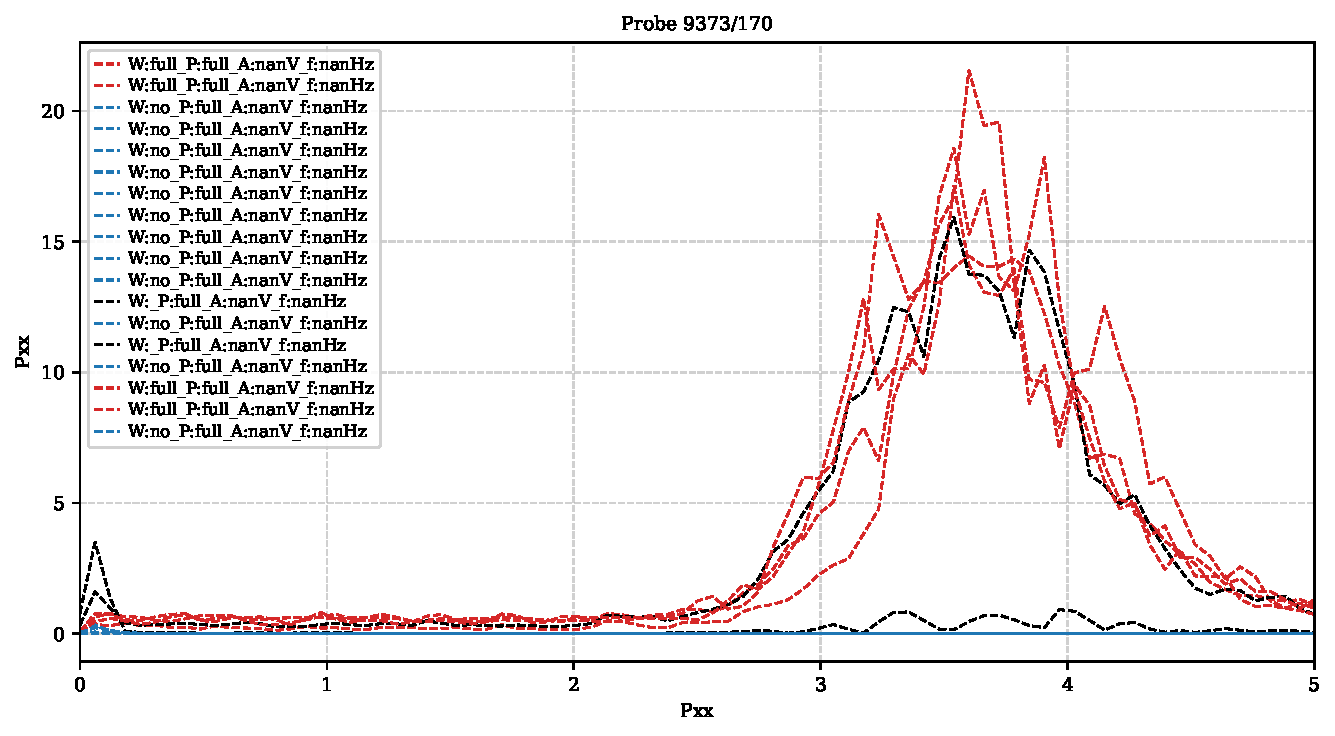
\includegraphics[width=\linewidth]{FIGURES/04_spectrum_psd_allpanel-allwind-ampallamp-freqallfreq-probe9373-170.pdf}
    \caption{TODO}
    \label{fig:TODO_9373}
  \end{subfigure}
  \hfill
  \begin{subfigure}[b]{0.48\linewidth}
    \centering
    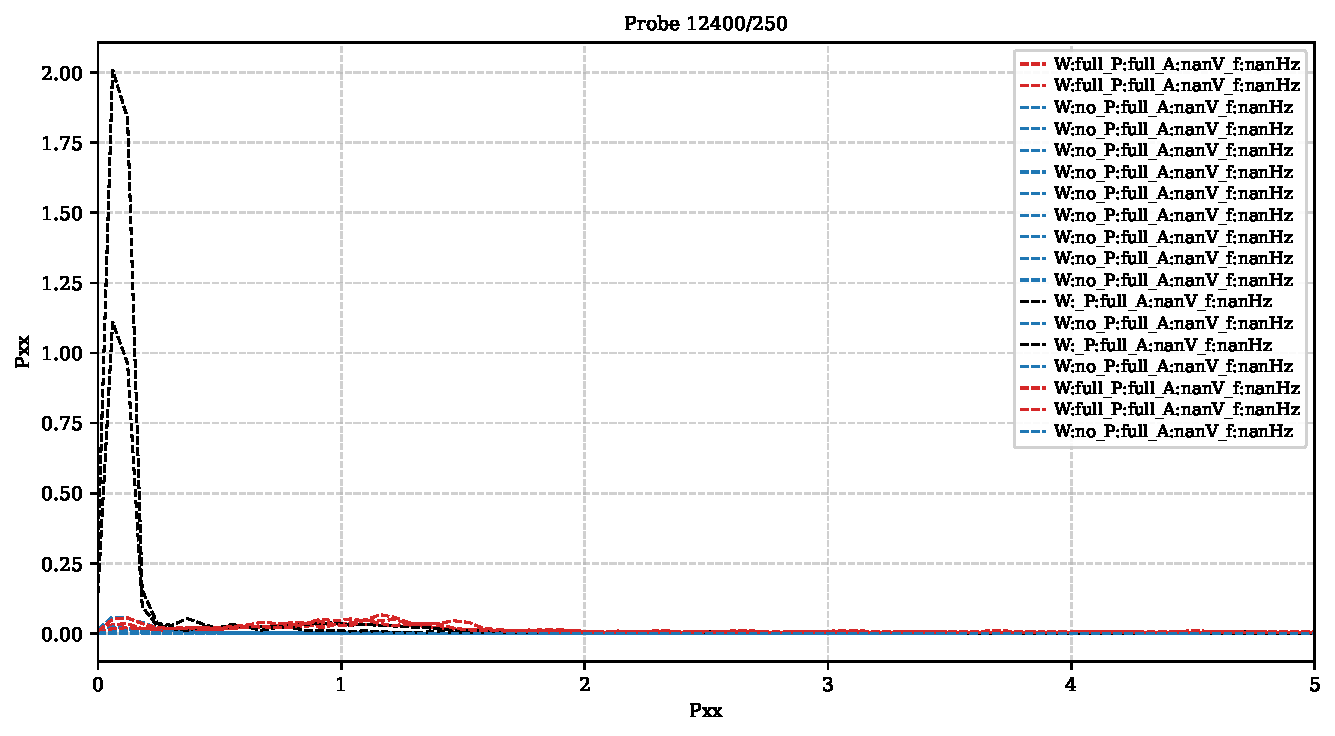
\includegraphics[width=\linewidth]{FIGURES/04_spectrum_psd_allpanel-allwind-ampallamp-freqallfreq-probe12400-250.pdf}
    \caption{TODO}
    \label{fig:TODO_12400}
  \end{subfigure}
  \hfill
  \begin{subfigure}[b]{0.48\linewidth}
    \centering
    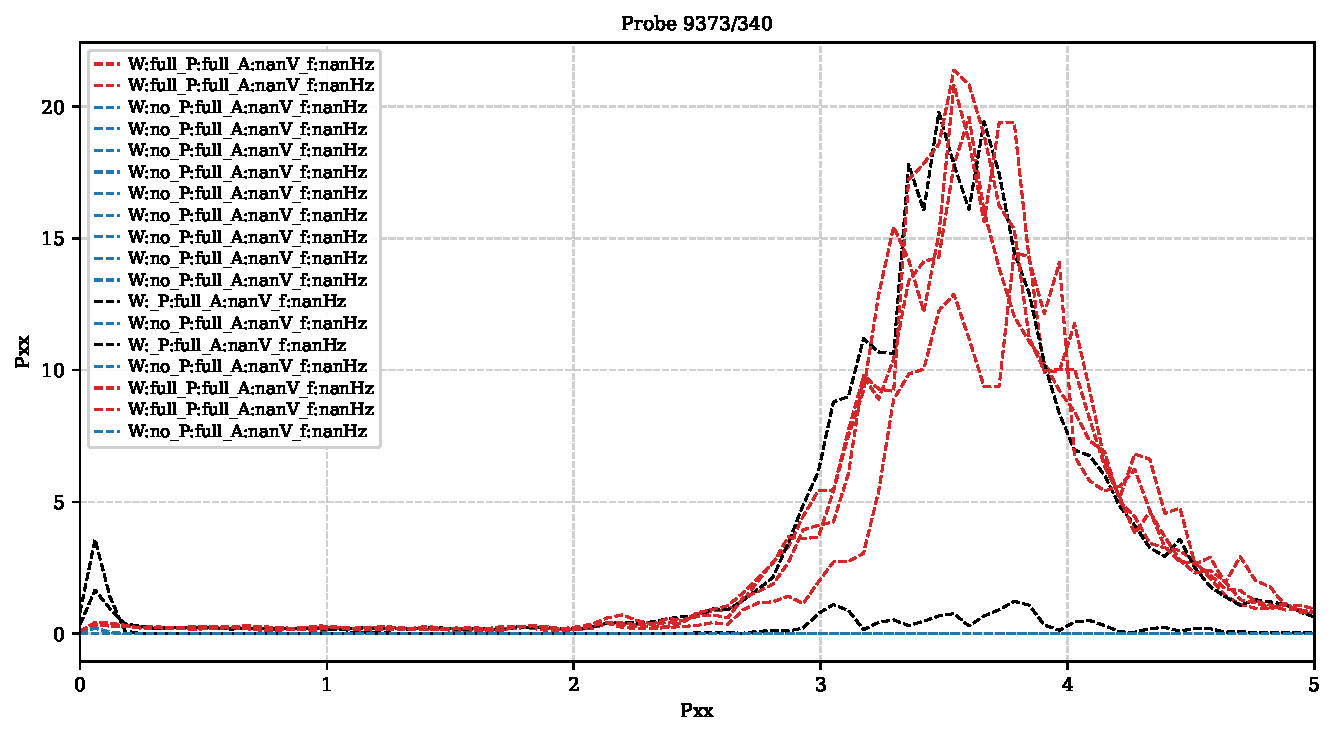
\includegraphics[width=\linewidth]{FIGURES/04_spectrum_psd_allpanel-allwind-ampallamp-freqallfreq-probe9373-340.pdf}
    \caption{TODO}
    \label{fig:TODO_9373}
  \end{subfigure}
  \hfill
  \begin{subfigure}[b]{0.48\linewidth}
    \centering
    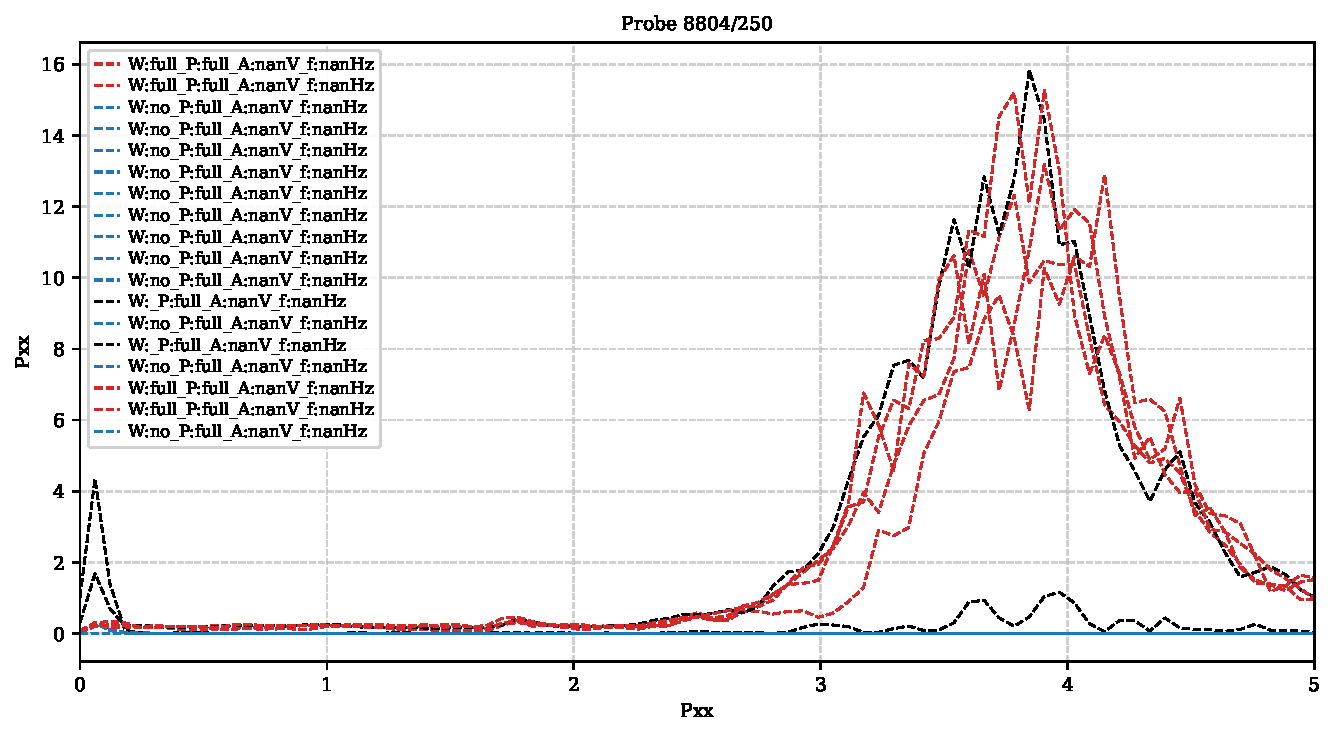
\includegraphics[width=\linewidth]{FIGURES/04_spectrum_psd_allpanel-allwind-ampallamp-freqallfreq-probe8804-250.pdf}
    \caption{TODO}
    \label{fig:TODO_8804}
  \end{subfigure}
  \caption[POWER spectral density (PSD) of the free surface at each wave gauge during wind-only runs (no paddle waves)]{
    POWER spectral density (PSD) of the free surface at each wave gauge during wind-only runs (no paddle waves). All 19 nowave runs overlaid; colour encodes wind condition. Stillwater runs (no wind) shown as baseline. Wind energy is concentrated above 2\,Hz — the paddle frequency range (0.65--1.9\,Hz) is unaffected.
  }
  \label{fig:ch04_wind_psd}
\end{figure}
